%Version 2.1 April 2023
% See section 11 of the User Manual for version history
%
%%%%%%%%%%%%%%%%%%%%%%%%%%%%%%%%%%%%%%%%%%%%%%%%%%%%%%%%%%%%%%%%%%%%%%
%%                                                                 %%
%% Please do not use \input{...} to include other tex files.       %%
%% Submit your LaTeX manuscript as one .tex document.              %%
%%                                                                 %%
%% All additional figures and files should be attached             %%
%% separately and not embedded in the \TeX\ document itself.       %%
%%                                                                 %%
%%%%%%%%%%%%%%%%%%%%%%%%%%%%%%%%%%%%%%%%%%%%%%%%%%%%%%%%%%%%%%%%%%%%%

%%\documentclass[referee,sn-basic]{sn-jnl}% referee option is meant for double line spacing

%%=======================================================%%
%% to print line numbers in the margin use lineno option %%
%%=======================================================%%

%%\documentclass[lineno,sn-basic]{sn-jnl}% Basic Springer Nature Reference Style/Chemistry Reference Style

%%======================================================%%
%% to compile with pdflatex/xelatex use pdflatex option %%
%%======================================================%%
 
\documentclass[sn-mathphys,Numbered]{sn-jnl}% Math and Physical Sciences Reference Style

%%%% Standard Packages
%%<additional latex packages if required can be included here>

\usepackage{makecell}
\usepackage{graphicx}%
\usepackage{multirow}%
\usepackage{amsmath,amssymb,amsfonts}%
\usepackage{amsthm}%
\usepackage{mathrsfs}%
\usepackage[title]{appendix}%
\usepackage{xcolor, soul}%
\usepackage{textcomp}%
\usepackage{manyfoot}%
\usepackage{booktabs}%
\usepackage{algorithm}%
\usepackage{algorithmicx}%
\usepackage{algpseudocode}%
\usepackage{listings}%
\usepackage{pdflscape}%
%%%%

%%%%%=============================================================================%%%%
%%%%  Remarks: This template is provided to aid authors with the preparation
%%%%  of original research articles intended for submission to journals published 
%%%%  by Springer Nature. The guidance has been prepared in partnership with 
%%%%  production teams to conform to Springer Nature technical requirements. 
%%%%  Editorial and presentation requirements differ among journal portfolios and 
%%%%  research disciplines. You may find sections in this template are irrelevant 
%%%%  to your work and are empowered to omit any such section if allowed by the 
%%%%  journal you intend to submit to. The submission guidelines and policies 
%%%%  of the journal take precedence. A detailed User Manual is available in the 
%%%%  template package for technical guidance.
%%%%%=============================================================================%%%%

%\jyear{2021}%

\DeclareRobustCommand{\hlcyan}[1]{{\sethlcolor{cyan}\hl{#1}}}


\raggedbottom
%%\unnumbered% uncomment this for unnumbered level heads

\begin{document}

\title[Labor productivity shifts during the electric vehicle transition: early evidence from case studies in the U.S.]{Labor productivity shifts during the electric vehicle transition: early evidence from case studies in the U.S.}

%%=============================================================%%
%% Prefix	-> \pfx{Dr}
%% GivenName	-> \fnm{Joergen W.}
%% Particle	-> \spfx{van der} -> surname prefix
%% FamilyName	-> \sur{Ploeg}
%% Suffix	-> \sfx{IV}
%% NatureName	-> \tanm{Poet Laureate} -> Title after name
%% Degrees	-> \dgr{MSc, PhD}
%% \author*[1,2]{\pfx{Dr} \fnm{Joergen W.} \spfx{van der} \sur{Ploeg} \sfx{IV} \tanm{Poet Laureate} 
%%                 \dgr{MSc, PhD}}\email{iauthor@gmail.com}
%%=============================================================%%

\author[1]{\fnm{Andrew} \sur{Weng}}\email{asweng@umich.edu}
\equalcont{These authors contributed equally to this work.}

\author[1]{\fnm{Omar} Y. \sur{Ahmed}}\email{oyahmed@umich.edu}
\equalcont{These authors contributed equally to this work.}

\author*[1]{\fnm{Anna} \sur{Stefanopoulou}}\email{annastef@umich.edu}

\affil[1]{\orgdiv{Department of Mechanical Engineering}, \orgname{University of Michigan - Ann Arbor}, \orgaddress{\street{1231 Beal Ave}, \city{Ann Arbor}, \postcode{48109}, \state{MI}, \country{U.S.}}}

\abstract{
As the world shifts towards a fully electrified transportation sector, a parallel transition in the labor market is unfolding in which millions of internal combustion engine vehicle (ICEV) assembly jobs are being replaced by jobs needed to produce and assemble battery electric vehicles (BEVs). A central question surrounding this transition remains contested: ``will the transition to BEVs lead to more or fewer manufacturing jobs?" This work uses publicly available datasets on vehicle production and employment to show that historic ICEV assembly plants in the U.S. that have fully transitioned to producing BEVs have required at least as many workers to produce the same number of vehicles. Our study suggests that loss of employment is not an inevitable outcome of the BEV transition. The methodology introduced here can be used as a general framework for monitoring and reporting regional labor market outcomes as the world transitions to full decarbonization. 
}

\keywords{electric vehicle manufacturing, manufacturing jobs, labor productivity, Just Transition}

\maketitle

\section{Introduction}


\begin{figure*}[tp!]
\centering
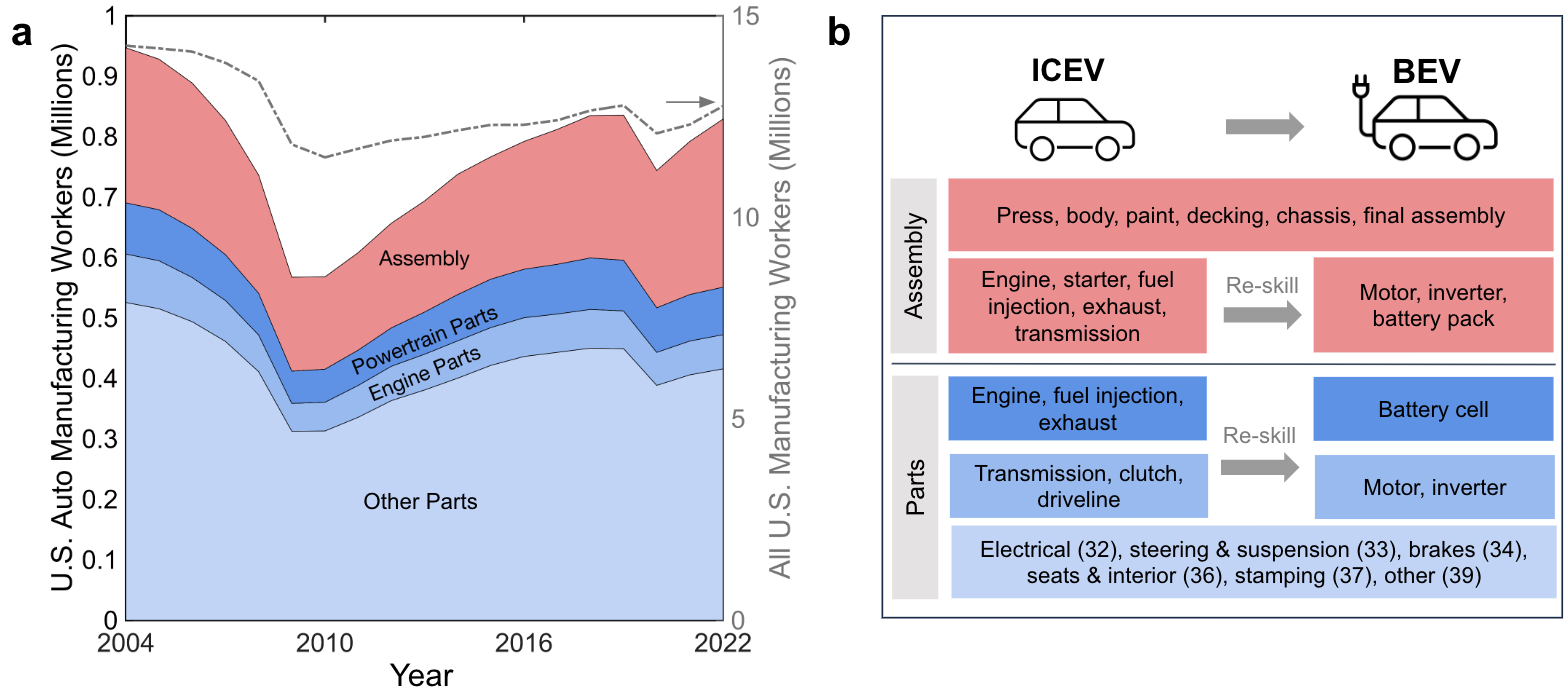
\includegraphics[width=1.0\linewidth]{figures/fig_overview.png}
\caption{(a) U.S. automotive sector employment consists of assembly and parts manufacturing jobs, with assembly comprising 33\% of total automotive jobs. During periods of economic downturn (e.g. the recession of 2008 and the pandemic of 2019), job loss rates in the automotive sector exceed that of the overall U.S. manufacturing sector (secondary y-axis). (b) The transition from ICEV to BEV production will create shifts in the types and quantities of jobs in both assembly and parts manufacturing. Instead of workers for the manufacturing and assembly of engines, BEVs will need workers for the manufacturing of battery cells and the assembly of battery packs. Assembly jobs: NAICS 3361. Engine parts jobs: NAICS 33631. Powertrain parts jobs: NAICS 33635. Other parts: NAICS codes 336(xx) according to the parenthesized values in (b).}
\label{fig:overview}
\end{figure*}

The automotive industry employs 13 million workers in the U.S.  including nearly 1 million in the manufacturing sector \cite{International_Labor_Organization2020-es, US_Bureau_of_Labor_Statistics2023-vr} (Figure \ref{fig:overview}a). While most of these workers are engaged in the production of internal combustion engine vehicles (ICEVs) today, a rapid shift towards battery electric vehicles (BEVs) is underway as major automakers set ambitious targets to phase out ICEV production within the next decade \cite{International_Energy_Agency2023-dd, National-Academies-2021}. As ICEV production ramps down, engine-related assembly and parts manufacturing jobs will be lost. In the place of these jobs, new jobs in electric motor and battery cell assembly and manufacturing will be created (Figure \ref{fig:overview}b).

How will the transition to BEV production affect the overall number of jobs in the automotive sector? The answer to this question is at the core of a Just Transition which ``secur[es] the future and livelihoods of workers and their communities in the transition to a low-carbon economy'' \cite{Emden2022-wa, Romero-Lankao2023-ws, Just_Transition_Initiative2021-mq, Lim2023-dp}. The notion of a Just Transition is especially salient in the U.S. where losing a job often means losing health care coverage \cite{Himmelstein2019-bm} and where unemployment insurance benefits fall below the poverty threshold for a family of three in most states \cite{DeSilver2020-oy, US_Department_of_Health_and_Human_Services_undated-my, Tasini2021-jk}. For many U.S. auto workers, the possibility of job loss is not theoretical but experienced. During the 2008 global recession, automotive manufacturing employment declined by 23\% within a year (Figure \ref{fig:overview}a). The automotive sector has been particularly vulnerable to job losses during periods of economic downturn compared to the overall U.S. manufacturing sector which lost fewer jobs (12\%) over the same period.

Despite the importance of understanding how BEV adoption will affect the quantity of automotive jobs, reports on this topic have been scarce and contradictory. A common narrative is that BEV powertrains have fewer parts compared to ICEV powertrains and thus take fewer workers to assemble, so the BEV transition will result in a net loss in automotive jobs. The claim of ``30\% fewer workers for EV assembly'' entered public discourse as early as 2017 \cite{Ford_Motor_Company2017-ps} and remains a central claim as part of ongoing debates on the effect of the BEV transition on jobs \cite{Vellequette2019-qu, Levin2022-kt, Charette2023-jy, Fichera2023-lg}. The Economic Policy Institute similarly found that, without policies promoting local production of electric vehicle powertrain components, 75,000 jobs could be lost in the U.S. by 2030. However, the same report also predicted that jobs could rise by 150,000 jobs given local production \cite{Barrett2021-gf}. Another study by the Boston Consulting Group found that BEV labor requirements are about 1\% less than those for ICEVs after accounting for all production process differences \cite{Kupper2020-rh}. Yet another study by Cotterman et al. found that the labor demand required for BEV powertrain manufacturing can be more than twice as high as that for ICEVs if battery cell manufacturing is included and when ``real-world'' industry shop floor data is used instead of academic models \cite{Cotterman2022-jt}\footnote{The authors found that public sources and models, such as the BatPaC model \cite{Argonne_National_Lab2022-xx}, underestimate the labor intensity for BEV manufacturing when compared to those calculated from industry data, suggesting that ``real-world'' BEV powertrain manufacturing complexities are not fully accounted for by the existing models.}. The lack of consensus from existing reports underscores the difficulty with estimating the future trajectory of BEV jobs which hinge on assumptions of labor demand and battery cell manufacturing location \cite{Cotterman2022-jt, Kupper2020-rh, Barrett2021-gf}\footnote{The location of battery cell manufacturing is particularly integral to whether jobs are gained or lost in the automotive sector \cite{De_Ruyter2022-xn, Barrett2021-gf, The_White_House2022-jy} motivating recent industrial policy action including the Inflation Reduction Act to onshore battery manufacturing \cite{US_Department_of_the_Treasury2023-by}.}. 

This work studies vehicle assembly sites that have already fully transitioned from ICEV production to BEV production. In all three assembly sites studied, our study found that BEV assembly employment exceeded ICEV employment after controlling for the number of vehicles produced. By focusing on studying data from existing assembly sites, this result reveals the effect of the ongoing BEV transition on automotive assembly jobs in the U.S. without needing \textit{a priori} assumptions of labor intensity. The result provides a preview of future employment for U.S. automotive assembly jobs which comprised 33\% of all automotive manufacturing workers in 2022 and has been a focal point of the jobs debate \cite{Ford_Motor_Company2017-ps} (Figure \ref{fig:overview}a). 
% Beyond considering whether the BEV transition will create or remove jobs, an equally important consideration is where the new jobs will be located \cite{Lim2023-dp}. A key detail in the Cotterman study was the inclusion of cell manufacturing as part of the labor intensity calculation for BEV powertrain manufacturing. In their study, cell manufacturing accounted for over 75\% of the total labor hours for BEV powertrain assembly \cite{Cotterman2022-jt}, with the rest being battery module and pack assembly. The inclusion of cell manufacturing in comparing the labor demand implies that net increases in employment may not be fully realized at the location of automakers if battery cell manufacturing does not occur at the same site. The importance of cell manufacturing location on where new automotive manufacturing jobs will be located is recognized by think-tanks and policy-makers alike as being a central component of a Just Transition \cite{De_Ruyter2022-xn, Barrett2021-gf, The_White_House2022-jy}.

% These aforementioned studies also underscore some of the existing difficulties in quantifying the effect of the BEV transition on labor productivity which we summarize here. First, BEV design and manufacturing technology, unlike those for ICEVs, remain in the early stages of technology development with processes yet to be optimized \cite{Degen2023-dt, Grant2022-re, Orum_Aydin2023-vg}. This fact is reflected by the average price of an electric vehicle which remains 24\% higher than for all passenger cars at the end of 2022 \cite{Ewing2023-vj}. Labor intensity for BEVs may thus decrease from today's reported values as EV manufacturing technology matures. Second, comparing labor intensity between BEV and ICEV requires identifying the scope of labor included as part of `parts assembly' specifically whether battery and cell manufacturing is included. As Cotterman et al. showed \cite{Cotterman2022-jt}, cell manufacturing is a major source of labor intensity for BEV production.


% \begin{figure*}[ht]
% \centering
% \includegraphics[width=1.0\linewidth]{figures/overview.png}
% \caption{Overview of the study. (A) Map of U.S. auto manufacturing activity as of 2022, featuring the number of workers classified under ``motor vehicle manufacturing'' (NAICS Code 3361) and manufacturing plants in each state. Three ``transition plants'' have been identified as examples of complete ICEV to BEV production transformations: (1) Alameda County, CA, representing the transition of the former New United Motors Manufacturing, Inc. (NUMMI) vehicle assembly plant, which assembled ICEV passenger vehicles, to the Tesla plant which assembles BEVs including the Model S, Model X, Model 3 and Model Y; (2) Oakland County, Michigan, representing the transition from the production of General Motors ICEVs to the Chevy Bolt BEV over the course of six years; and (3) McLean County, Illinois, representing the transition of the former Mitsubishi vehicle assembly plant to the Rivian plant which assembles electric pick-up trucks. (B) Comparison of similarities and differences between ICEV and BEV assembly including parts assembly and parts manufacturing. (C) Vehicle production history for each of the three transition plants.}
% \label{fig:overview}
% \end{figure*}

\section{Identifying BEV transition plants}

We focus this study on U.S. counties in which there exists a single historic site of ICEV assembly which has since been repurposed to produce BEVs (Figure \ref{fig:assembly}a). These sites, termed ``transition plants,'' provide the most direct comparison of labor intensity differences before, during, and after the BEV transition, and are defined by three attributes. First, the site must have fully transitioned from the assembly of ICEVs to BEVs. A full transition ensures that the latest labor productivity figures fully correspond to BEV production without considering the effect of parallel production of BEV and ICEVs. Second, the site must have been producing BEVs for at least two years and at a volume of more than 10,000 vehicles per year. These filters exclude BEV assembly plants that are in the very early stages of production ramp-up where production volumes are far from equilibrium conditions\footnote{Note that, even after 2 years of production, steady-state volume production is still not guaranteed, a factor that we will later address.}. 


\begin{figure*}[tp!]
\centering
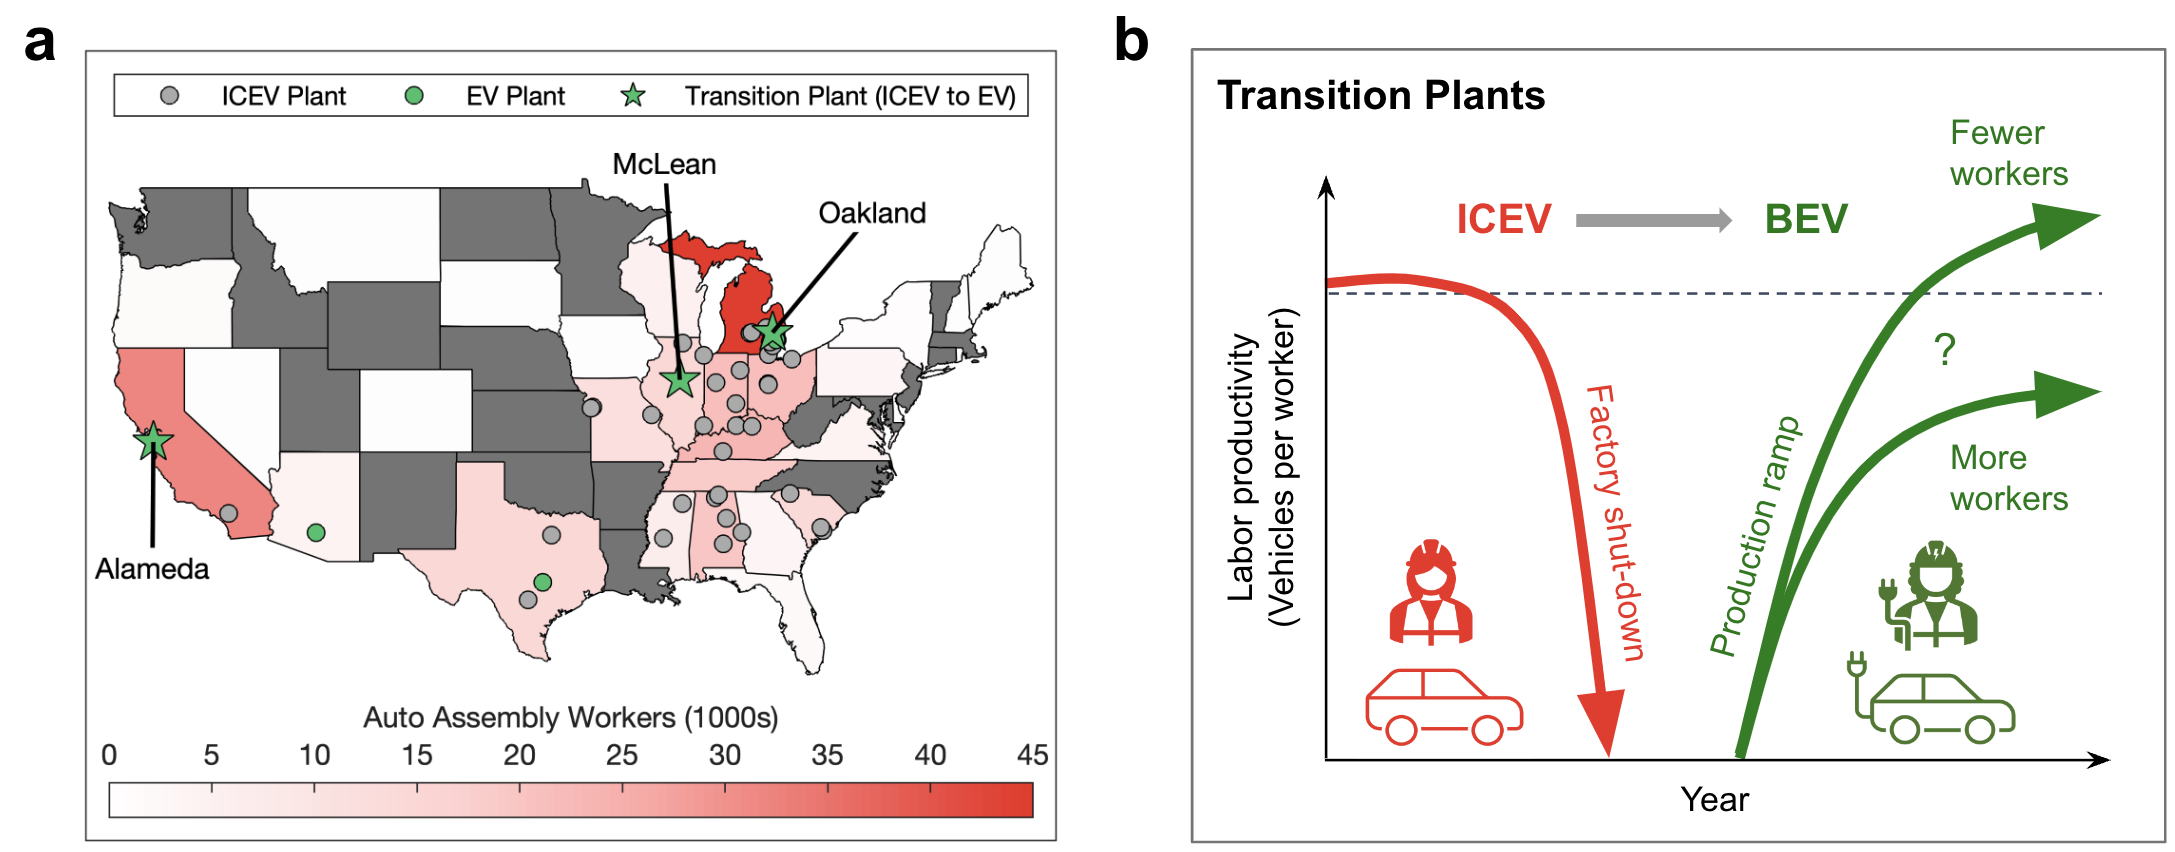
\includegraphics[width=1.0\linewidth]{figures/fig_assembly.png}
\caption{Studying sites of vehicle assembly that have fully transitioned from assembling ICEVs to assembling BEVs (``transition plants''). (a) Map of U.S. automotive vehicle assembly activity as of 2022. Colors show the number of workers classified under ``motor vehicle manufacturing'' (NAICS code 3361) for each state. Markers highlight major manufacturing plants in each state. Three ``transition plants'' have been identified as examples of complete ICEV to BEV production transformations: (1) Alameda County, CA, representing the transition of the former New United Motors Manufacturing, Inc. (NUMMI) vehicle assembly plant, which assembled ICEV passenger vehicles, to the Tesla plant which assembles BEVs; (2) Oakland County, Michigan, representing the transition from the production of General Motors ICEVs to the Chevy Bolt BEV over six years; and (3) McLean County, Illinois, representing the transition of the former Mitsubishi vehicle assembly plant to the Rivian plant which assembles electric pick-up trucks. (b) Idealized trajectory of vehicle assembly labor productivity before, during, and after the BEV transition.}
\label{fig:assembly}
\end{figure*}

We identify three transition plants for this study: Oakland County in Michigan, Alameda County in California, and McLean County in Illinois. Oakland is home to the General Motors (GM) Orion assembly plant which began producing the Chevy Bolt BEV in 2016 concurrently with ICEVs but has since transitioned to producing only the Bolt as of 2021 \cite{Burden2016-pg}. Oakland thus provides a case study in which the same workforce transitioned from making ICEVs to making BEVs over a period of five years. Alameda was next chosen as the site of the historic New United Motor Manufacturing Incorporated (NUMMI) plant, a joint venture between General Motors and Toyota, which closed in 2010 and has since been operated by Tesla to make BEVs. Alameda represents a `near-steady-state' BEV assembly case: Tesla has now been producing BEVs from this site for over a decade and its annual production volume of BEVs now exceeds that of the NUMMI plant at its peak. Finally, McLean was included as a third transition plant. McLean is the home to a former ICEV plant owned by Mitsubishi which has since been taken over by Rivian to produce mass-market electric light-duty trucks. McLean represents the case of a burgeoning BEV manufacturer at the early stages of production ramp-up.

\section{Understanding employment potential through labor productivity}

At each transition plant, we study the labor productivity before, during, and after the transition to BEVs according to: 
\begin{equation}
    P(y) = \frac{V(y)}{W(y)},
\end{equation}
where $P$ is the site's labor productivity, $V$ is the total number of light-duty vehicles produced at the site, and $W$ is the number of auto assembly workers employed at the site averaged over four quarters of each year. Each quantity is defined for each year $y$. Higher labor productivity implies that fewer workers are needed to produce each vehicle, and vice versa. Figure \ref{fig:assembly}b highlights how labor productivity is expected to shift during the BEV assembly. First, labor productivity drops to zero as ICEV production ramps down. Next, as historical vehicle lines are retooled for assembling BEVs, labor productivity gradually ramps. Eventually, BEV assembly labor productivity reaches a steady-state value through learning. new assembly processes stabilize. 

Vehicle production data is obtained from Automotive News Research \& Data Center \cite{Automotive_News2023-pg} which details vehicle production volumes per make, model, and assembly location (see Section \ref{sec:veh}). Automotive assembly worker data reflects employment under the North American Industrial Classification System (NAICS) code 3361 and is collated from publicly available government data and news reports (see Section \ref{sec:emp}). U.S. national level vehicle production, assembly workers, and labor productivity are provided in Figure \ref{fig:us-metrics}. Notably, since BEV uptake has not surpassed 7\% of the total vehicle market in the U.S. as of 2022, these macro-level trends represent primarily activity from ICEV-producing assembly plants and can thus be used as baseline trends for studying individual site-level differences. Note that labor productivity at the U.S. level ranged between 40 and 60 vehicles per worker, with productivity tending to increase following periods of economic downturn (i.e. after the 2008 Great Recession and after the 2021 COVID-19 pandemic). 

% Another related metric is the labor intensity $L$ defined as
% \begin{equation}
%     L = \frac{t_\mathrm{worked}}{P}
% \end{equation}
% where $L$ is the number of hours it takes to build one vehicle and $t_\mathrm{worked}$ is the annualized number of hours spent per employee. $t_\mathrm{worked}$ is estimated to be 2236 hours assuming an average of 43 hours worked per week for vehicle manufacturing workers according to BLS \cite{US_Bureau_of_Labor_Statistics2022-zg}.

\section{Alameda: doubling of workers per vehicle after a decade of BEV production}

Alameda County, California, is home to the historic vehicle assembly plant formerly owned by North America Motor Manufacturing Incorporated (NUMMI) \cite{Austenfeld2007-db}. The plant was in operation from 1984 to 2010 as a joint venture between General Motors and Toyota, producing ca. 430,000 vehicles per year at its peak. The plant produced both passenger vehicles (Toyota Corolla and Pontiac Vibe) as well as light-duty trucks (Toyota Tacoma) (Figure \ref{fig:alameda}a). The plant closed in 2010 after General Motors pulled out of the partnership amidst the global recession \cite{Shaiken2010-bn, Troncoso2012-hv}. The plant closure resulted in the direct loss of 4,700 manufacturing jobs \cite{Shaiken2010-bn} as well as the closure of 34 businesses in Alameda that supplied parts to the factory \cite{Johnston2015-zh}. 

\begin{figure*}[tp!]
\centering
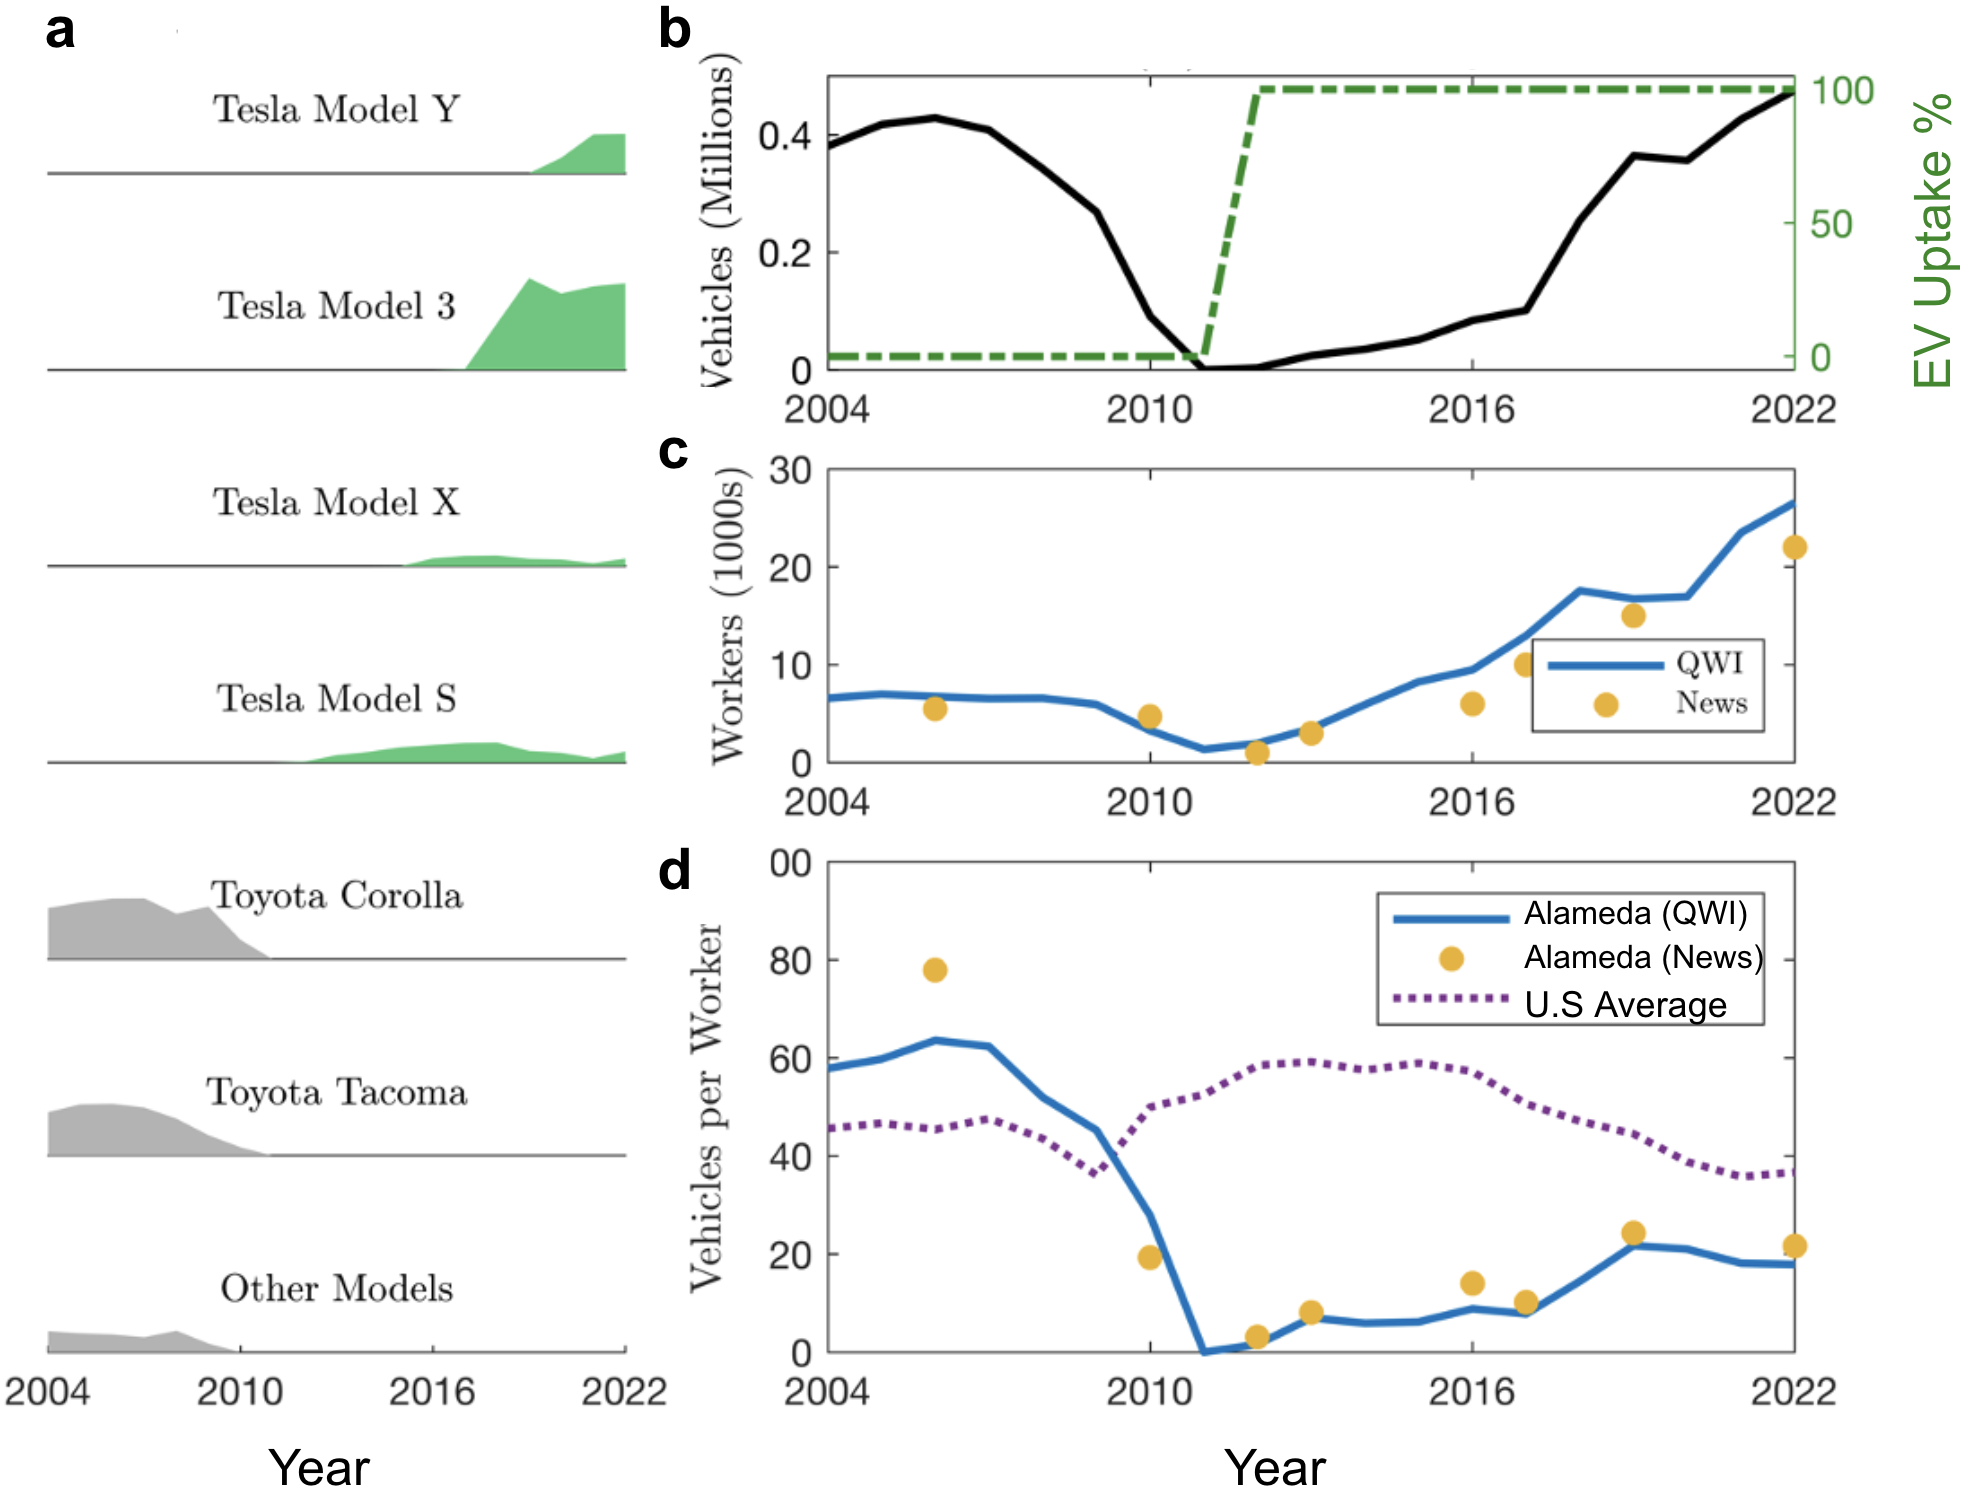
\includegraphics[width=1.0\linewidth]{figures/fig_alameda.png}
\caption{(a) Vehicle production history in Alameda County, California. Before 2010, the New United Motors Manufacturing Incorporated (NUMMI) factory produced passenger sedans. The factory has since been taken over by Tesla which has now been producing BEVs for over a decade. (b) Annual vehicle production volumes. (c) Employment numbers according to the U.S. Quarterly Wages Indicator (QWI) under NAICS classification 3361 and news reports. (d) Labor productivity of assembly workers in Alameda Co. compared to the U.S. average.}
\label{fig:alameda}
\end{figure*}

% Before the plant closure, the factory operated with two shifts per day, five days per week \cite{Solman2010-rw}.

Following the NUMMI plant closure, Tesla purchased the factory and began to retool the lines, first to produce the Model S and X luxury sedan and SUV starting in 2012 and 2015, respectively, followed by the Model 3 and Y mass-market vehicles starting in 2017 and 2020, respectively. By 2019, annual vehicle production volume in the Tesla plant surpassed that of the NUMMI plant at its peak, and by 2022, the plant was producing more than 450,000 units per year (Figure \ref{fig:alameda}b). Over the past decade, Tesla has maintained a hiring rate of ca. 2,500 manufacturing workers per year, totaling over 25,000 workers as of 2021 (Figure \ref{fig:alameda}c). These employment numbers are corroborated by both governmental data (QCEW) and by local new reports (Appendix \ref{sec:news-reports}).

The NUMMI factory reached peak labor productivity in 2006 at 66 vehicles per worker which also coincided with peak annual vehicle production (Figure \ref{fig:alameda}d). Since this peak, labor productivity began to decline year-on-year along with vehicle production volume. By 2012, vehicle production was effectively zero, representing a total loss in factory productivity as the NUMMI plant was shut down. After Tesla purchased the factory and began to build the Model S in 2012, labor productivity began to rise but saturated at ca. 10 vehicles per worker over the next five years. Labor productivity rose again starting in 2017 when Tesla began production of the Model 3, its mass-market BEV. During this period, labor productivity peaked at ca. 25 vehicles per worker. Overall, during the decade since Tesla began to build BEVs, labor productivity never exceeded 22 vehicles per worker. 

In summary, Tesla employed at least twice as many workers to produce each BEV between 2012 and 2022 compared to ICEVs made in the same factory under the ownership of NUMMI between 2004 and 2008. To the best of our knowledge, this BEV labor force in Alameda includes labor for battery pack assembly for the Model S and Model X \cite{Cohen2014-tx} but excludes battery pack assembly for the Model 3 and Model Y which are reportedly manufactured off-site in Reno, Nevada \cite{Field2019-dw, Hawley2023-ek, Kane2022-cp, The_Tesla_Team2017-cp, Korosec2017-kd}. The BEV in Alameda labor force further excludes the labor for battery cell manufacturing which has been reported to account for up to 75\% of total labor needed to make a BEV powertrain \cite{Cotterman2022-jt}. Battery cells for the Tesla Model S and X are sourced from Panasonic in Japan \cite{The_Tesla_Team2011-ua} and cells for the Tesla Model 3 and Y are reportedly made in a factory in Reno, Nevada \cite{Field2019-dw, Hawley2023-ek, Kane2022-cp, The_Tesla_Team2017-cp}. Starting in 2017, Tesla also began to make Model 3 electric motors \cite{Lambert2016-ds, Korosec2017-kd} and battery packs in Gigafactory 1 located in Sparks, Nevada. The data after 2017 thus primarily reflects the labor productivity for assembling Model 3 and Y vehicles excluding electric motor manufacturing, battery cell manufacturing, and most of battery pack manufacturing\footnote{While Model S/X pack assembly purportedly takes place in Alameda, S/X vehicle sales only account for x\% of total vehicle sales}. When employment numbers from Sparks, Nevada are included, labor productivity decreases further to 15 vehicles per worker (Figure \ref{fig:alameda-cell}).

Overall, the NUMMI-Tesla transition highlights one example of an ICEV to BEV transition in which BEVs took more than twice as many workers to assemble, even before considering the additional labor needed to manufacture battery cells and electric motors. Tesla, now with more than a decade of BEV production, has reached annual production volumes exceeding its former ICEV counterparts. Yet, labor productivity in the factory, at ca. 25 vehicles per worker, remains far from the peak productivity realized by the NUMMI plant in 2006 which exceeded 60 vehicles per worker.


\section{Oakland: similar vehicle architecture, similar employment}

Oakland County, Michigan, is the home to the Orion Assembly plant owned by General Motors (GM). Before the 2008 recession, the plant produced the Chevy Malibu and Pontiac G6 passenger sedans with production volumes exceeding 450,000 per year in 2005 (Figure \ref{fig:oakland}a). Production numbers declined in the proceeding years, eventually reaching zero in 2008 when the plant was idled as GM declared bankruptcy \cite{Goldstein2017-cm} (Figure \ref{fig:oakland}b). As the economy recovered from the recession, the Orion plant re-opened to produce the Buick Verano and Chevy Sonic passenger sedans \cite{Vlasic2011-hc, Nadrowski2011-xq}. Then in 2016, GM began to convert its assembly lines to produce the Chevy Bolt BEV \cite{Burden2016-pg}. By 2021, the plant has fully transitioned to assembling the Chevy Bolt EV, though total production numbers never exceeded 50,000 units per year. Motor vehicle assembly employment in Oakland County throughout these periods mirrored the vehicle production numbers: as vehicle production declined, so did employment (Figure \ref{fig:oakland}c).


\begin{figure*}[tp!]
\centering
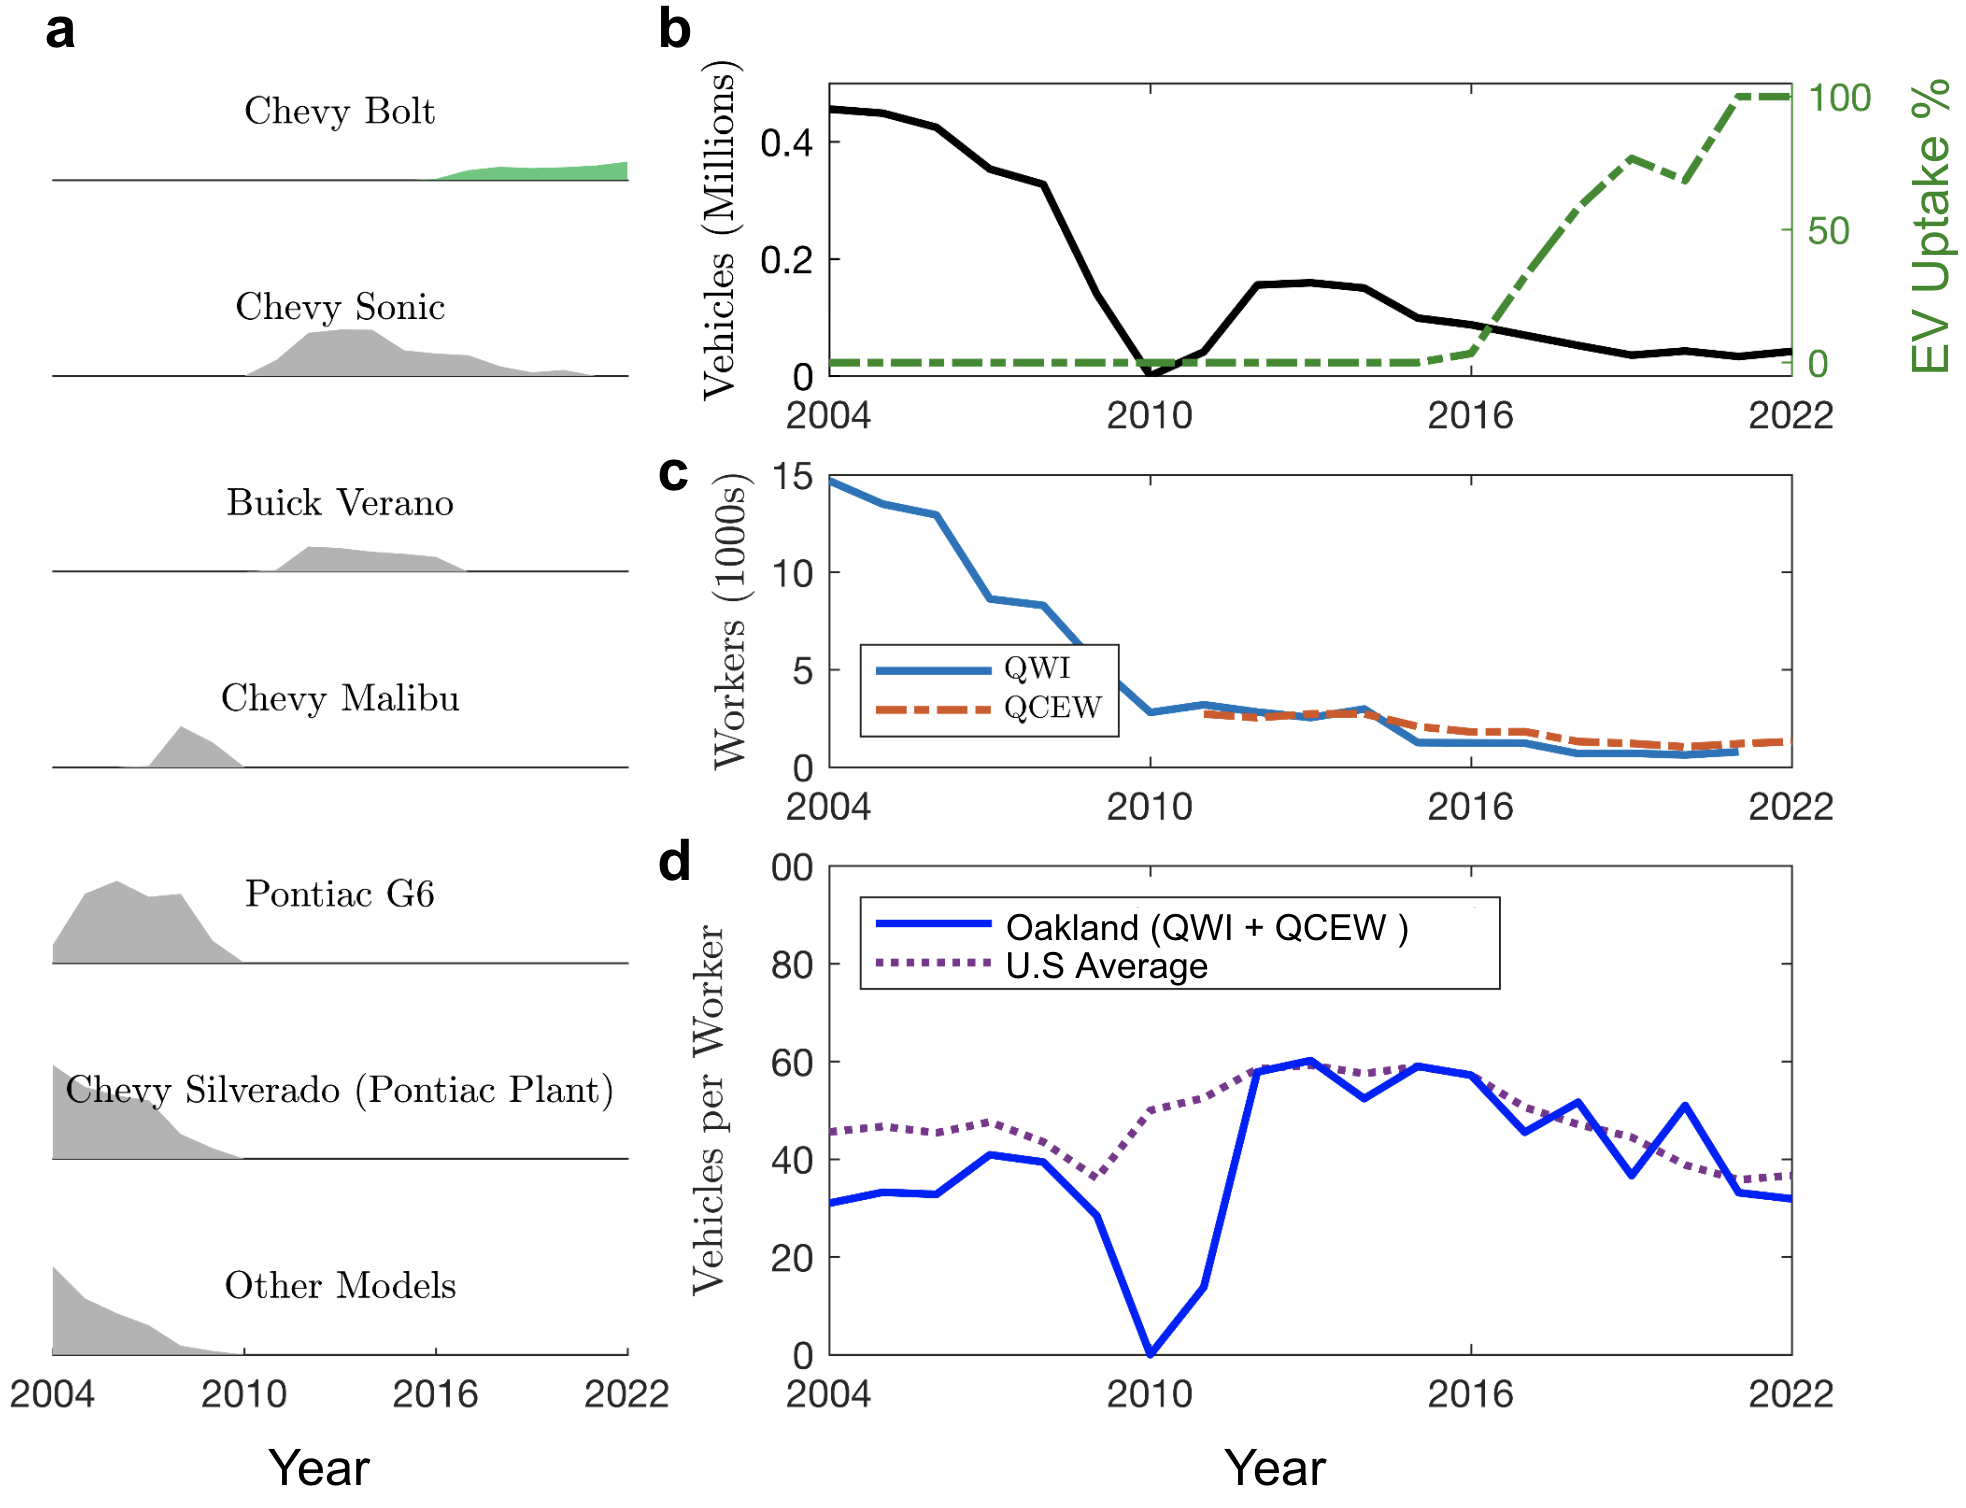
\includegraphics[width=1.0\linewidth]{figures/fig_oakland.png}
\caption{(a) Vehicle production history in Oakland County, Michigan, home to the Orion Township assembly plant owned by General Motors. Before the 2008 recession, plants in the cities of Pontiac and Wixom were also actively producing vehicles, but both plants shut down in 2010, leaving the Orion plant as the sole operating plant in the county. Before 2010, the New United Motors Manufacturing Incorporated (NUMMI) factory produced passenger sedans. The factory has since been taken over by Tesla which has now been producing BEVs for over a decade. (b) Annual vehicle production volumes. (c) Employment numbers according to the U.S. Quarterly Wages Indicator (QWI) under NAICS classification 3361 and news reports. (d) Labor productivity of assembly workers in Oakland Co. compared to the U.S. average.}
\label{fig:oakland}
\end{figure*}


To understand the labor productivity of BEV assembly, we focus on the years 2021 and 2022 in Figure \ref{fig:oakland}d. During these years, only the Chevy Bolt BEV was produced. The labor productivity of assembling ICEVs can be found from data before 2016 when the factory was making only ICEVs. During this period, labor productivity varied widely (Figure \ref{fig:oakland}d). Before the 2008 recession, vehicles per worker stayed below 40. During GM's bankruptcy in 2010, labor productivity reached zero since the factory shut down. However, by 2013, labor productivity surpassed levels before the recession, peaking at 62 vehicles per worker. Finally, as the plant began to transition to making the Chevy Bolt BEV, labor productivity began to decline again. By 2022, when the plant was only making Chevy Bolt BEVs, labor productivity was 38 vehicles per worker, on par with the labor productivity for ICEV assembly before the 2008 recession. Moreover, labor productivity in 2022 was also on par with the U.S. average trend which reflects predominantly ICEV production during the same period. Altogether, the results suggest that the Chevy Bolt does not take more labor to assemble than compared to ICEV counterparts.  %During the transition to the Chevy Bolt, the number of shifts in this factory was reduced from two to only one, a common practice in many factories during times of economic strain \cite{Intelligence2023-qt}

Overall, the transition to making the Chevy Bolt BEV did not appreciably change the labor productivity in Oakland. Oakland thus represents a case where the transition to BEV production resulted in a similar number of jobs per vehicle produced. Note that, while jobs per vehicle remained similar, the total number of jobs declined due to the decline in vehicle production volumes (Figure \ref{fig:oakland}b,c). Finally, we note that the labor productivity corresponding to Chevy Bolt BEV assembly excludes battery pack assembly labor to the best of our knowledge\footnote{Battery pack assembly occurs at a separate facility in Hazel Park, Michigan. The economic output of the Hazel Park facility is not vehicles and is assumed to be excluded from NAICS code 3361 (motor vehicle manufacturing)}. Battery cell manufacturing labor is similarly excluded since the battery cells are manufactured off-site\footnote{The battery cells for the Chevy Bolt BEV are made by LG in South Korea or Holland, Michigan\cite{Motors2021-mf, Motors2021-bm}. However, note that, for newer GM BEVs, such as the Hummer EV and the Cadillac Lyriq, battery pack assembly and vehicle assembly are planned to occur at the same location. These new production sites are excluded from this study since no data is available yet.}. Labor productivity is expected to decrease if either battery pack assembly or cell manufacturing activity is included.

\section{McLean: ten-fold employment increase during BEV factory production ramp}

In this final case study, we turn to McLean County, Illinois, home to the former Mitsubishi vehicle assembly plant \cite{Motors2004-cc} (Figure \ref{fig:normal}). During Mitsubishi's ownership, the plant produced models including the Eclipse sedan and Outlander sport utility vehicle with peak annual vehicle production reaching 68,000 vehicles in 2014. In the same year, the plant employed 1,250 workers. In 2015, Mitsubishi shut down operations due to global competitive pressures \cite{Yerak2015-kk}. The plant was subsequently purchased by Rivian to build electric pickup trucks \cite{The_Detroit_News2022-ym}. In 2022, Rivian produced 24,000 electric vehicles while employing 6,000 workers. 


\begin{figure*}[ht]
\centering
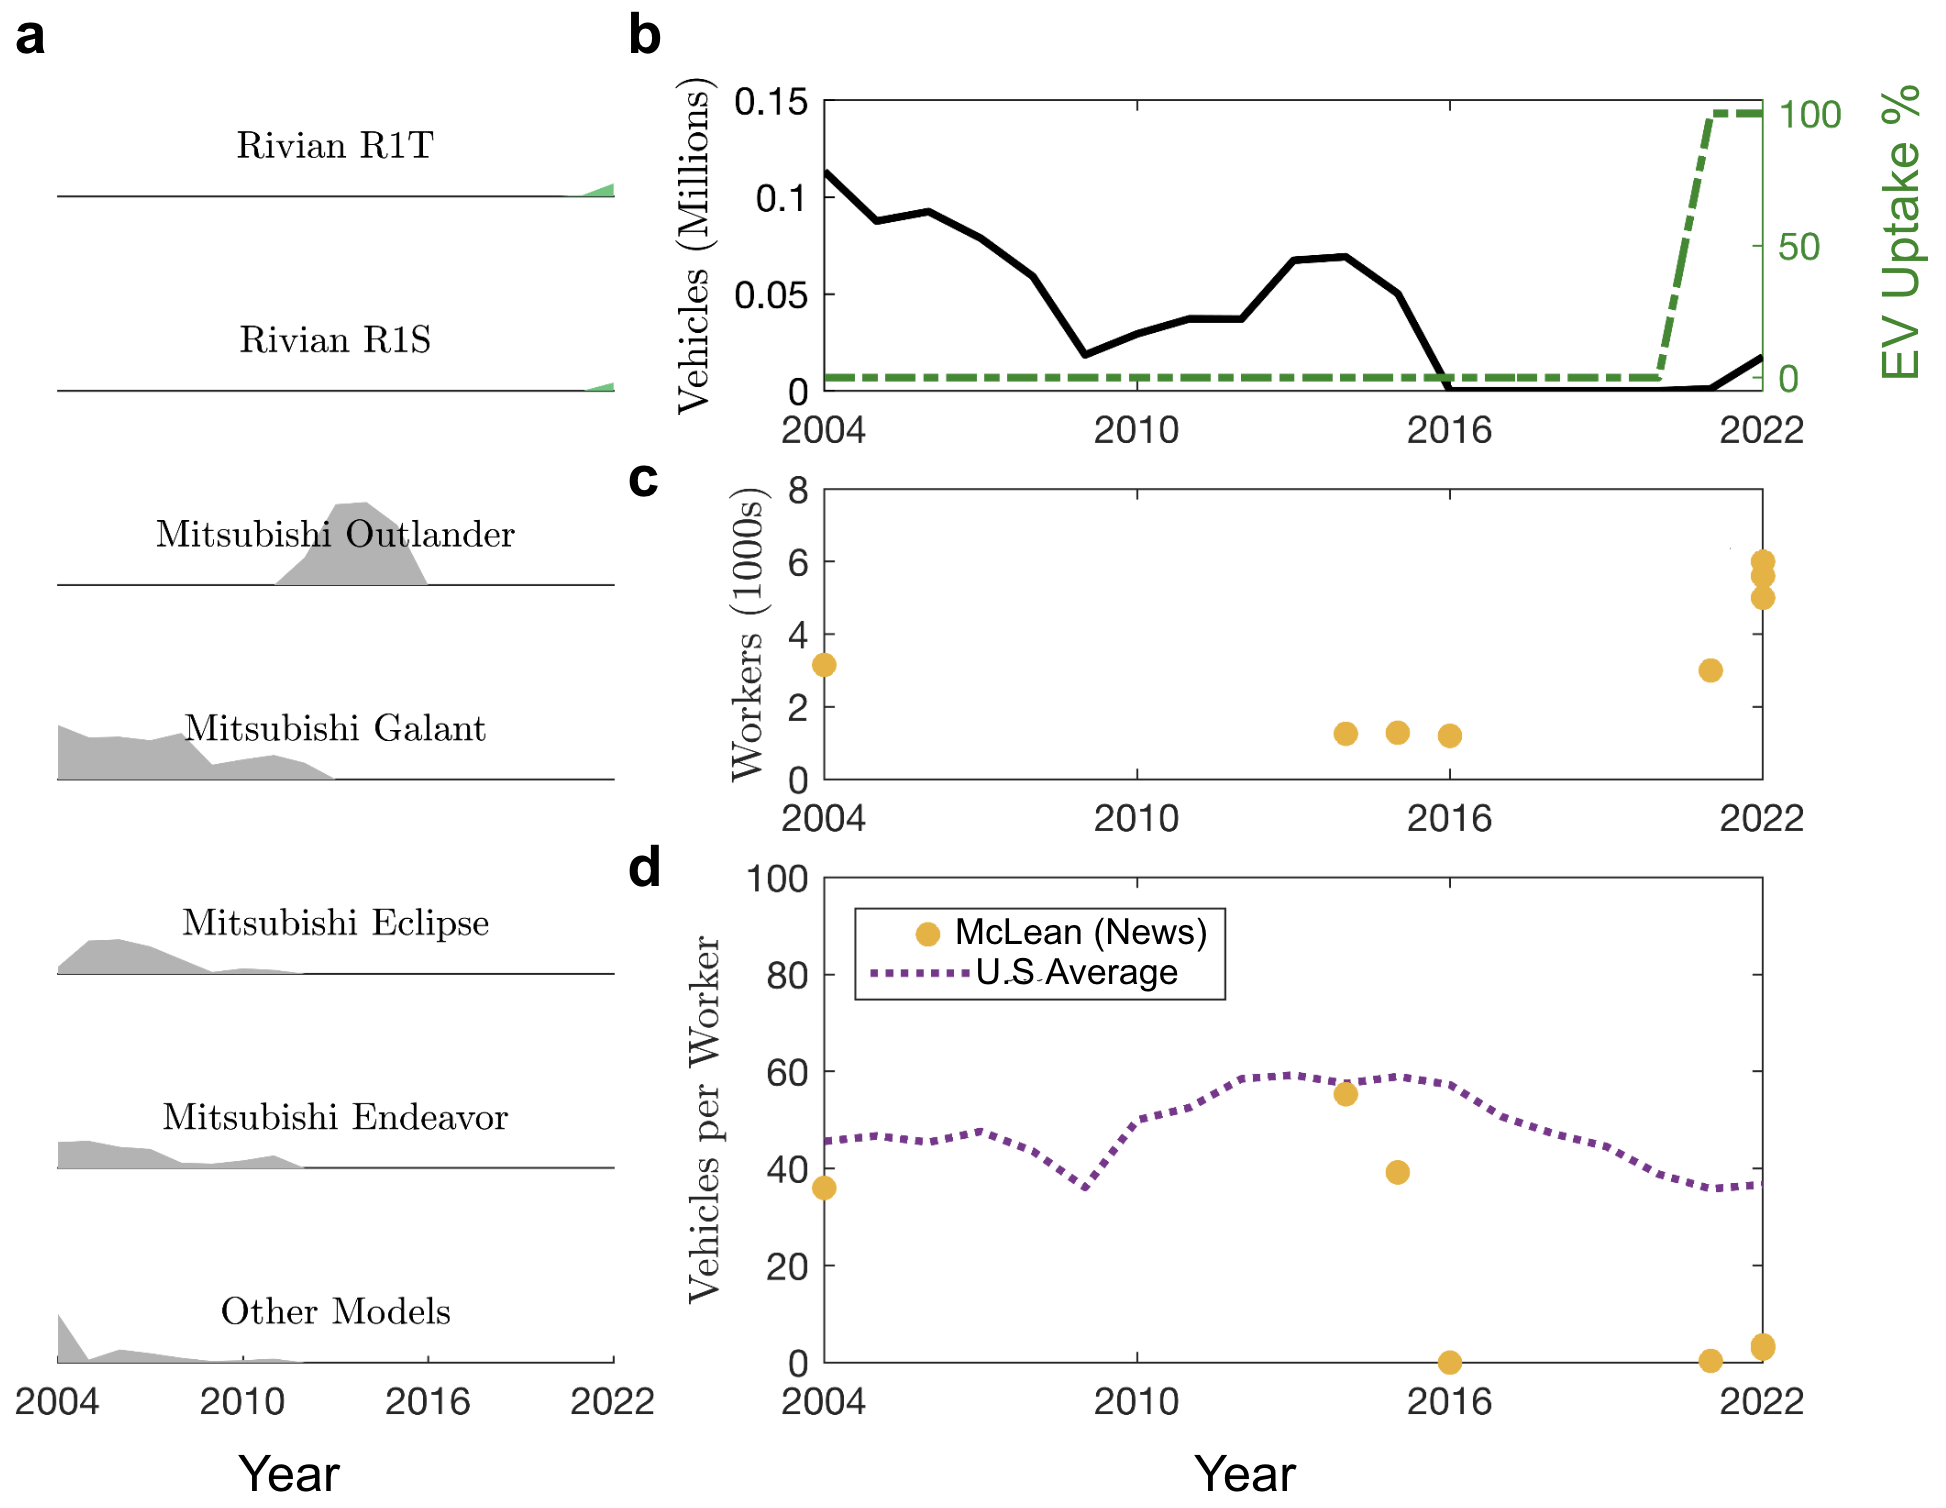
\includegraphics[width=1.0\linewidth]{figures/fig_mclean.png}
\caption{(a) Vehicle production history in McLean County, Illinois. Before 2016, Mitsubishi owned an ICEV production plant in the town of Normal. The factory has since been taken over by Rivian which began producing electric SUVs and pick-up trucks in 2021. (b) Annual vehicle production volumes. (c) Employment numbers according to news reports. Employment data from the U.S. government, including QWI and QECW, was not available for this county due to data suppression. (d) Labor productivity of assembly workers in McLean Co. compared to the U.S. average.}
\label{fig:normal}
\end{figure*}

Overall, labor productivity was 47 vehicles per worker during ICEV production in 2014 compared to 2.5 vehicles per worker during BEV production in 2022. The low labor productivity seen in 2022 mirrors the similarly low level seen during Alameda's first five years of BEV production (Figure \ref{fig:alameda}d). Both cases represent periods during which fledgling BEV makers undergo rapid production ramp-up and where production levels have not yet reached steady state. Rivian also reportedly manufactures battery packs on-site \cite{Weintraub2021-ti}, contributing to an additional source of labor burden which is included in the labor productivity calculation. Note, however, that the battery cells used by Rivian are made by Samsung, are not manufactured on-site \cite{Weintraub2021-ti}, and thus do not contribute to the labor productivity calculation.

\section{Discussion}

The three case studies in Alameda, Oakland, and McLean counties collectively suggest that BEVs take just as many, if not more, workers to assemble than ICEVs. We reiterate this finding in Table \ref{tab:productivity-summary} which highlights, for each transition plant, the peak labor productivity before and after the BEV transition. Here, we introduce a metric, ``workers per 1,000 vehicles'' (WPV), the inverse of vehicles per worker, which provides a direct measure of employment normalized against production volume. In Alameda, WPV rose three-fold from 15 to 46 after the BEV transition. In Oakland, WPV rose from 16 to 26. Finally, in McLean, WPV rose from 18 to 250. In all three cases, the number of workers per vehicle increased following the BEV transition.

\begin{table}
    \centering
    \begin{tabular}{rcc}
        & Pure ICEV Assembly Case & Pure BEV Assembly Case \\
        \toprule        
        \multicolumn{1}{l}{\textbf{Alameda, CA}} & & \\
        Owner & NUMMI & Tesla \\
        Vehicle models & Tacoma, Corolla, Vibe & Model S/X/3/Y \\
        Peak productivity year & 2006 & 2019 \\
        Labor productivity & 66 vpw & 22 vpw \\
        Workers / 1000 vehicles & \textbf{15} & \textbf{46} \\
        Production volume & 426,000 & 362,000 \\
        Employment & 6,500 & 16,600 \\
        Includes pack assembly? & - & Some* \\
        Includes cell manuf.? & - & No \\
        \midrule
        \multicolumn{1}{l}{\textbf{Oakland, MI}} & & \\
        Owner & General Motors & General Motors \\
        Vehicle models & Sonic, Verano, Malibu, G6 & Chevy Bolt EV \\
        Peak productivity year & 2013 & 2022 \\
        Labor productivity & 62 vpw & 38 vpw \\
        Workers / 1000 vehicles & \textbf{16} & \textbf{26} \\
        Production volume & 160,000 & 42,000 \\
        Employment & 2,600 & 1,100 \\
        Includes pack assembly? & - & No \\
        Includes cell manuf.? & - & No \\
        \midrule
        \multicolumn{1}{l}{\textbf{McLean, IL}} & & \\
        Owner & Mitsubishi & Rivian \\
        Vehicle models & Outlander, Galant, Eclipse & R1T, R1S \\
        Peak productivity year & 2014 & 2022 \\
        Labor productivity & 54 vpw & 4 vpw \\
        Workers / 1000 vehicles & \textbf{18} & \textbf{250} \\
        Production volume & 68,000 & 24,000 \\
        Employment & 1,250 & 6,000 \\
        Includes pack assembly? & - & Yes \\
        Includes cell manuf.? & - & No \\
        \bottomrule
    \end{tabular}
    \caption{More workers per vehicle needed for BEV assembly for all three counties studied. Productivity, production volume, employment numbers, and workers per vehicle metrics correspond to the year of peak labor productivity. The lists of vehicle models highlight certain high-volume production models and are not exhaustive. vpw: vehicles per worker.}
    \label{tab:productivity-summary}
\end{table}

Alameda highlights a labor productivity scenario for a maturing BEV assembly process. The fact that, after ten years of BEV production, WPV in Alameda remained more than twice as high compared to prior ICEV production in the same facility is thus perhaps surprising considering the common assumption that BEVs have fewer components than ICEVs should thus take less labor to assemble. The lowered labor productivity of BEV assembly in Alameda is further corroborated by comparing against the U.S. average value for automotive assembly during the same period which primarily reflects ICEV labor productivity as of 2022 (Figure \ref{fig:alameda}d). This comparison shows that labor productivity in Alameda remained 40\% lower than the U.S. average, i.e. most other ICEV production labor productivity occurring over the same period. We attribute the lowered labor productivity in Alameda partly to Tesla's approach to vertical integration which involves designing and manufacturing vehicle components in-house, including electric motors \cite{Bellon2022-wx}, semiconductors \cite{Cohen2014-tx} and seats \cite{Field2019-mi}. In contrast, legacy automakers, over a period between the late 1990s and early 2000s, have opted for a strategy of outsourcing in which many vehicle components such as the engine and transmission are designed and manufactured off-site by parts suppliers \cite{Cutcher-Gershenfeld2015-pv, Chen2019-qr}. From this perspective, the reduction in labor productivity seen in the BEV assembly figures in Alameda could indicate a trend towards a growing co-location of workers who have historically worked off-site (i.e. at the site of parts suppliers) who now work within the assembly plant (Figure \ref{fig:vertical-integration}). By comparison, parts manufacturing workers along the ICEV value chain (e.g. engine and transmission manufacturing workers), not being co-located in the vehicle assembly site, are not counted in the vehicle assembly labor productivity calculation. We finally note that Tesla's investment in manufacturing technology development \cite{Cutcher-Gershenfeld2015-pv} may also necessitate a larger workforce of salaried engineers who may be co-located within the same factory \cite{Furr2020-hr} which would further increase the workforce size at the site of vehicle assembly.

While this study focused on the trajectory of automotive assembly jobs which comprised 33\% of all auto manufacturing jobs in the U.S. in 2022 (Figure \ref{fig:overview}a), the fate of automotive parts jobs requires further study. With the BEV transition, some parts manufacturing jobs, particularly in engine manufacturing, will inevitably be lost. In some cases they have already been lost, as is the case with South Australia \cite{De_Ruyter2022-xn}. In the U.S., engine manufacturing jobs accounted for x\% of all U.S. auto manufacturing jobs in 2022, or y workers. Will the BEV transition create more jobs to replace those that are lost? 

A major source of BEV labor intensity is battery cell manufacturing. Cotterman et al. estimated that cell manufacturing may account for up to 75\% of the total labor intensity for producing a BEV powertrain \cite{Cotterman2022-jt}. Public data on Tesla employment also suggests that battery cell manufacturing including pack assembly can increase labor needed per BEV by over 50\%: in 2022, Alameda employed 22,000 workers for vehicle assembly, and in the same year, Tesla and Panasonic Energy of North America (the cell supplier) jointly employed 12,000 workers to manufacture cells and assemble battery packs. In other words, for every two workers needed to assemble a BEV, an additional worker is needed to manufacture the battery cells and build the battery pack.

Ultimately, whether new jobs in battery cell manufacturing will be able to replace lost jobs in automotive parts manufacturing depends on three attributes: (1) labor needed to make battery cells, (2) geographical co-location of jobs, and (3) skills needed. 


\begin{itemize}
\item Comparison of skills for ICE vs EV \cite{Cotterman2022-yb}
\item Skill demands and mismatch in U.S. manufacturing \cite{Weaver2017-dx}
\item Role of skills in manufacturing innovation, focusing on suppliers \cite{Helper2016-gb}
\item ``The myth of education:'' the overriding factor in jobs today is based not on competition over skills but competition based on wages \cite{Tasini2021-jk}.
\item Where are all the good jobs going? \cite{Kalleberg2013-wd}
\end{itemize}

% \subsection{The Role of Technology Innovation in the Resurgence of the Automotive Industry}

% ``In the last two decades, the U.S. auto industry has been shaped by globalization and the associated arrival of transplants. These forces have caused the geography of the U.S. auto industry to undergo a dramatic transformation. They have also had important effects on the wages and benefits of the domestic auto manufacturers and on their supply chains.'' \cite{Cutcher-Gershenfeld2015-pv}

% ``An appreciation of the auto industry today and in the future is inextricably entwined with the advances of technology'' \cite{Cutcher-Gershenfeld2015-pv}

% ``The larger trends related to transplants and shifting industry geography obscure a number of additional shifts in the supply chains. First, in the late 1990s and early 2000s, there was a move by all three of the major U.S. original equipment manufacturers to outsource many aspects of component design to suppliers. This was seen as a cost-saving move, with the companies focusing on what they termed their “core” business. This strategy proved problematic, however, as key knowledge within the OEMs on the component designs dissipated, reducing the ability to oversee the work. As costs and warranty issues with component parts began to mount, the OEMs have begun to bring more engineering and design work in-house.'' \cite{Cutcher-Gershenfeld2015-pv}

Socially responsible automation highlights the social importance of expanding labor productivity metrics beyond cost-based metrics \cite{Sampath2018-bo}.

\begin{figure*}[ht]
\centering
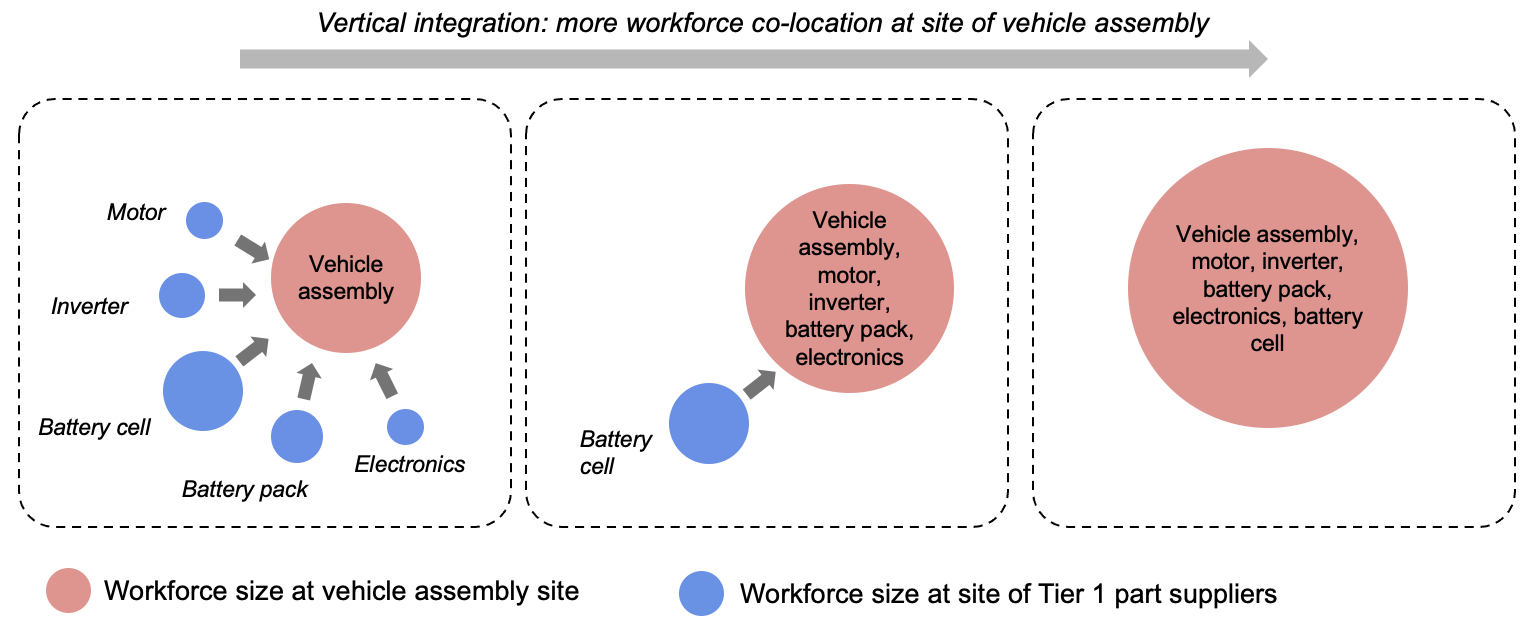
\includegraphics[width=1\linewidth]{figures/fig_vertical_integration.png}
\caption{Concept illustration: vertical integration creates more workforce co-location at the site of vehicle assembly.}
\label{fig:vertical-integration}
\end{figure*}


\begin{figure*}[ht]
\centering
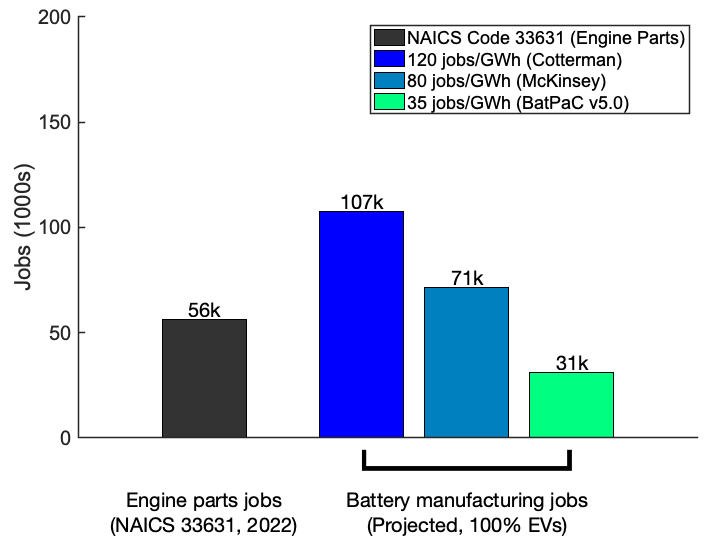
\includegraphics[width=0.8\linewidth]{figures/fig_engine_parts.png}
\caption{Comparison of engine manufacturing parts jobs in 2022 against projected battery cell manufacturing jobs assuming 100\% BEV uptake and under various assumptions of jobs per GWh.}
\label{fig:engine-jobs}
\end{figure*}


\section{Methods}

\subsection{Vehicle Production Data}
\label{sec:veh}

Vehicle production data $V$ was obtained from the Automotive News Research \& Data Center \cite{Automotive_News2023-pg} which collates North American light-duty (i.e., passenger vehicles and pick-up trucks) vehicle sales, production, and inventory data on a monthly basis and organizes the data by automaker, vehicle make and model, and manufacturing plant location. Only vehicle production in the U.S. was considered for this work. Electric vehicle models were manually identified by cross-referencing publicly available lists of BEV makes and models. The counties in which manufacturing plants reside were manually identified using the counties' Federal Information Processing System (FIPS) codes to enable linking county-level employment data with vehicle production data (see Section \ref{sec:emp}).

\subsection{Employment Data}
\label{sec:emp}

Automotive manufacturing employment data $W$ was obtained by cross-referencing three data sources: the Quarterly Census of Employment and Wages (QCEW), Quarterly Workforce Indicators (QWI), and local news reports. 

The QCEW dataset, administered by the U.S. Bureau of Labor Statistics (BLS), consists of a quarterly count of employment and wages for workers covered by unemployment insurance programs, which results in more than 95\% of U.S. jobs of workers \cite{Sadeghi2008-km}. QCEW thus encompasses nearly all employers in the U.S., which accounts for approximately 97\% of employees. The data is aggregated and classified by industry according to the North American Industry Classification System (NAICS), and provided for county, metropolitan statistical area (MSA), state, and national levels. This dataset provides employment data at the level of ``establishments'', defined as a single physical worksite engaged, predominantly, in one type of economic activity, e.g. making automotive vehicles.

The QWI dataset is administered by the U.S. Census Bureau and consists of administrative data from the Longitudinal Employer-Household Dynamics (LEHD) program, including Unemployment Insurance Wage Records, data from the Census Bureau, and data from the Office of Personnel Management (OPM). This allows the QWI dataset to provide both firm-level and worker-level data. The QWI data covers more than just those eligible for unemployment insurance benefits and includes all employers and their employees for which the administrative records are available. It provides detailed breakdowns by worker demographics (gender, age, education, race, and ethnicity), as well as earnings, and various measures of job and worker flows. Unlike QCEW which focuses on the establishment level, QWI produced insights into both the employer side (job creation, destruction, etc.) and employee side (turnover rates, accessions, separations) of labor dynamics.

For both the QCEW and QWI datasets, employment numbers were provided at a state and county level, classified by industry according to the North American Industry Classification System (NAICS). Specifically, NAICS code 3361 corresponds to Motor Vehicle Manufacturing. These codes were used to identify the number of employees belonging to business establishments involved in motor vehicle manufacturing. Parts manufacturing is excluded from these counts. 

Finally, local news reports, found via internet searches, provided another independent estimate of employment data for specific automotive factory sites. This data was used to corroborate existing QCEW data and QWI data or to substitute employment data where QCEW and QWI data are both unavailable.

\subsection{Limitations}

Regional employment data from QCEW and QWI is often suppressed to maintain employer anonymity. This most often occurs when a single large employer comprises a majority of the data for a particular industry in a particular region.

Another limitation is that employment data corresponding to NAICS code 3361 covers both light- and heavy-duty vehicle manufacturing employment. The vehicle production data from Automotive News only covers light-duty vehicles, so combining the two datasets requires assuming a negligible volume of heavy-duty vehicle manufacturing presence within the selected counties. NAICS sub-code 33611 covers employment specifically for light-duty manufacturing but the data is suppressed.

In most cases, the employment numbers from these data sources agree with each other, improving confidence in the reported numbers. 

Another common input for labor productivity calculations is the total number of hours worked. While this input is annually measured at the national level through surveys such as Current Employment Statistics (CES), county-level data is not made public by government agencies. For this reason, we used the number of workers as the input when calculating labor productivity.

\section*{Resource Availability}

Further information and requests should be directed to and will be fulfilled by Anna Stefanopoulou (\url{annastef@umich.edu}).

\section*{Acknowledgements}

The authors thank Kristin Dziczek for her insights and guidance on the auto manufacturing landscape in Michigan. The authors also thank Katelyn Freese and Katerina Freudenberg for their assistance with processing vehicle production data.

\section*{Author Contributions}

A.W.: methodology; writing - original draft; writing - review and editing; resources. O.Y.A: methodology; software; data curation; visualization; writing - original draft; writing - review and editing. A.S: conceptualization; writing - review and editing; funding acquisition.

\section*{Glossary of Terms}
\begin{tabular}{ l l }
    BEV & Battery Electric Vehicle \\
    GM & General Motors \\
    ICEV & Internal Combustion Engine Vehicle \\
    NAICS & North American Industry Classification System \\
    NUMMI & New United Motors Manufacturing Inc. \\
    QCEW & Quarterly Census on Employment and Wages \\
    QWI & Quarterly Wages Indicator 
\end{tabular}


%%===========================================================================================%%
%% If you are submitting to one of the Nature Portfolio journals, using the eJP submission   %%
%% system, please include the references within the manuscript file itself. You may do this  %%
%% by copying the reference list from your .bbl file, paste it into the main manuscript .tex %%
%% file, and delete the associated \verb+\bibliography+ commands.                            %%
%%===========================================================================================%%

\clearpage

\bibliography{main}% common bib file
%% if required, the content of .bbl file can be included here once bbl is generated
%%\input sn-article.bbl

\clearpage

\begin{appendices}

% \section{U.S. Level Automotive Productivity Trends}
% \label{sec:us-level}

% Figure \ref{fig:us-level}A shows vehicle production trends in the U.S. over the last two decades. The decrease in 2008 coincided with the global recession and the decrease in 2020 coincided with the international Covid pandemic. While the pandemic appeared to suppress vehicle production, the decline in vehicle production began years earlier, at around 2016.

% The percentage of the total vehicle production that comprises EVs in the U.S. stayed below 1\% throughout the first half of the 2010's. Between 2017 and 2022, however, this number rose from 1\% to 7\%.

% Figure \ref{fig:us-level}B shows the labor productivity defined as annual number of vehicles produced per employee. Before the recession, productivity ranged between ca. 50 and 60 vehicles per employee. During the 2008 recession, this number decreased to 40. However, as the global economy recovered, productivity peaked at 70 vehicles per employee. However, after 2016, productivity began to steadily decline, reaching an all-time low in 2021 at ca. 35 vehicles per employee.

\section{Supplemental Figures}

\begin{figure*}[ht]
\centering
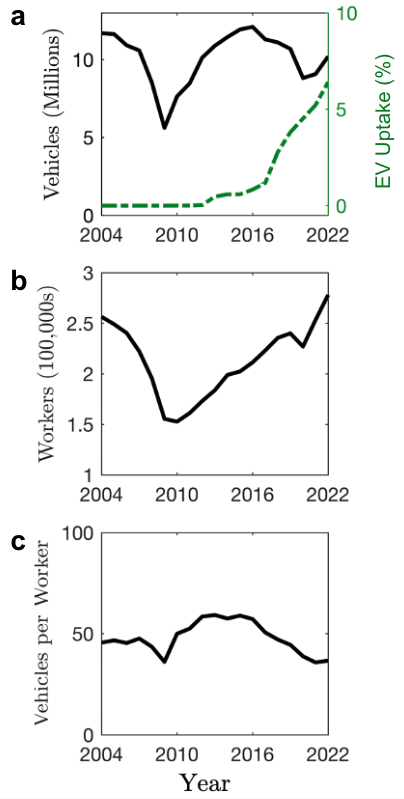
\includegraphics[width=0.6\linewidth]{figures/fig_us_metrics.png}
\caption{U.S.-level vehicle production (a), assembly workers (b), and labor productivity (c). }
\label{fig:us-metrics}
\end{figure*}

\begin{figure*}[ht]
\centering
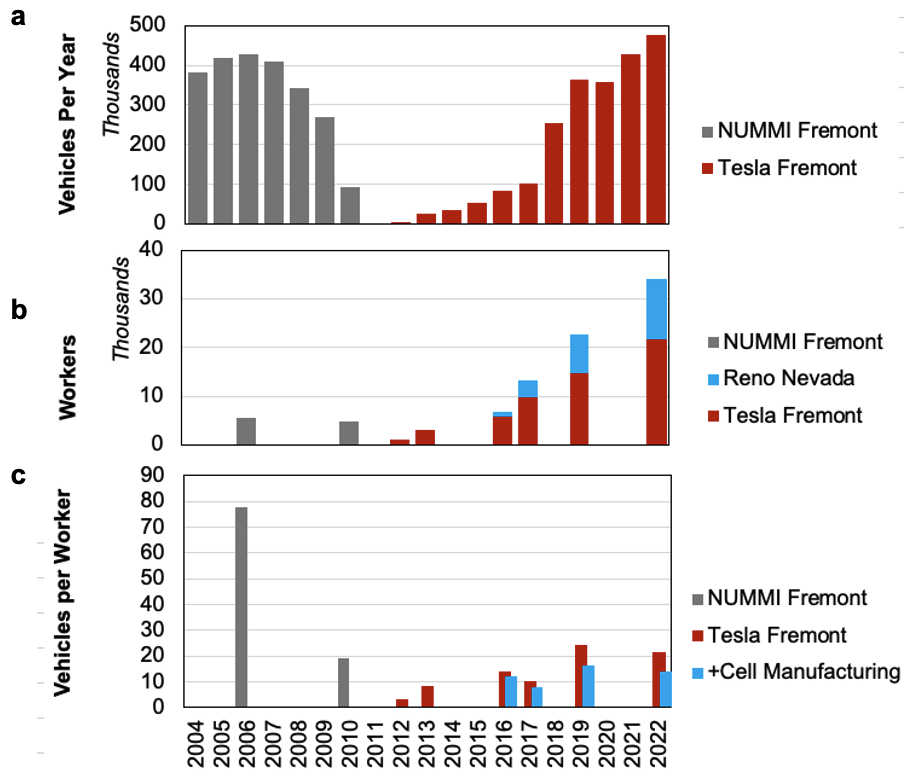
\includegraphics[width=1.0\linewidth]{figures/fig_alameda_reno.png}
\caption{(a) Vehicle production history in Alameda County, California. (b) Annual vehicle production volumes. (c) Employment numbers according to the U.S. Quarterly Wages Indicator (QWI) under NAICS classification 3361 and news reports. (d) Labor productivity of assembly workers in McLean Co. compared to the U.S. average.}
\label{fig:alameda-cell}
\end{figure*}


\label{sec:news-reports}

\begin{table}[ht]
    \centering
    \begin{tabular}{lclcc}
        Location & Date & News Source & Reported Employment \\
        \toprule
        Tesla (Alameda) & Jun 2012 & \href{https://www.sfgate.com/business/article/Tesla-starts-delivery-out-of-former-Nummi-plant-3653530.php}{SFGATE} & 1,000 \\
         & Jul 2013  & \href{https://www.wired.com/2013/07/tesla-plant-video/}{Wired} & 3,000 \\
         & Jun 2016 & \href{https://web.archive.org/web/20160716082915/http://www.thecountrycaller.com/40182-tesla-motors-tsla-workers-being-contacted-by-uaw-for-union-formation/}{TheCountryCaller} & 6,000 \\
         & Oct 2017 & \href{https://www.mercurynews.com/2017/10/13/4819750/}{The Mercury News} & 10,000 \\
         & Mar 2019 & \href{https://www.forbes.com/sites/alanohnsman/2019/03/01/tesla-safety-violations-dwarf-big-us-auto-plants-in-aftermath-of-musks-model-3-push/?sh=66dae5a454ce}{Forbes} & 15,000 \\
         & Jun 2022 & \href{https://web.archive.org/web/20220628005146/https://www.tesla.com/factory}{Tesla} & 22,000 \\
         \midrule 
        Tesla/PENA (Sparks) & 2016 & \href{https://electrek.co/2016/12/08/tesla-gigafactory-workers-2017-production-ramp-up/}{Electrek} & 850 \\
         & 2017 & \href{https://electrek.co/2018/08/21/tesla-gigafactory-1-3000-workers/}{Electrek} & 3,249 \\
         & 2018 & \href{https://apnews.com/general-news-2ffa3542a4b948c990f2f49ffd40621d}{The Associated Press} & 7,059 \\
         & 2022 & \href{https://web.archive.org/web/20191031042238/http://www.diversifynevada.com/wp-content/uploads/2018/07/2019_1001_NRS-360.975-3.5b-Tesla-Annual-Report.pdf}{Tesla} & 12,000 \\
        \midrule
         NUMMI (Alameda) & Jan 2002 & \href{https://www.sfgate.com/bayarea/article/Nummi-workers-say-their-final-good-byes-3194045.php}{SFGATE} & 5,739 \\ 
         & Mar 2006 & \href{https://www.eastbaytimes.com/2006/03/05/nummi-plant-a-model-for-ailing-car-industry/}{East Bay Times} & 5,500 \\
         & Apr 2010 & \href{https://www.recordnet.com/story/news/2010/04/02/end-nummi/51640719007/}{Recordnet.com} & 4,700 \\
         \midrule
         Rivian (Normal) & Oct 2021 & \href{https://www.wglt.org/local-news/2021-10-11/rivian-tops-3-000-workers-at-plant-in-normal}{WGLT} & 3,000 \\
         & Apr 2022 & \href{https://www.centralillinoisproud.com/news/local-news/report-rivian-reportedly-planning-layoffs/}{CIPROUD} & 5,000 \\
         & Jun 2022 & \href{https://energynews.us/2022/06/06/a-decade-after-evtown-rivian-is-making-an-illinois-citys-electric-vehicle-vision-a-reality/}{Energy News Network} & 5,600 \\
         & Jul 2022 & \href{https://www.centralillinoisproud.com/news/local-news/report-rivian-reportedly-planning-layoffs/}{CIPROUD} & 6,000 \\
         & Mar 2023 & \href{https://www.wglt.org/local-news/2023-03-16/rivian-growth-boosts-bloomington-normal-jobs-numbers}{WGLT} & 7,400 \\
         \midrule
         Mitsubishi (Normal) & 2004 & \href{https://www.chicagotribune.com/business/ct-mitsubishi-normal-0725-biz-20150724-story.html}{Chicago Tribune} & 3,150 \\ 
         & 2014 & \href{https://localwiki.org/bloomington-normal/Mitsubishi}{Local Wiki} & 1,250 \\
         & 2015 & \href{https://www.chicagotribune.com/business/ct-mitsubishi-normal-0725-biz-20150724-story.html}{Chicago Tribune} & 1,280 \\
         & 2016 & \href{https://www.wqad.com/article/news/local/drone/8-in-the-air/mitsubishi-motors-in-illinois-is-officially-closed/526-efeb1f03-c794-42ba-8128-596954a229da}{WQAD8} & 1,200 \\
         \midrule
         GM (Orion) & 2013 & \href{https://www.cargroup.org/wp-content/uploads/2017/02/Economic-Contribution-of-General-Motors-Orion-Assembly-Pontiac-Metal-Stamping-and-Spring-Hill-Assembly-Manufacturing-Plant.pdf}{CarGroup.org} & 2,561 \\
         & 2022 & \href{https://www.gm.com/company/facilities/orion}{GM} & 1,238 \\
         & 2023 & \href{https://www.wardsauto.com/industry-news/gm-path-electric-future-leads-through-detroit-area-plant}{Wards Auto} & 1,270 \\
         \bottomrule
    \end{tabular}
    \caption{List of news reports used to corroborate factory employment numbers. PENA: Panasonic Energy of North America.}
    \label{tab:news-reports}
\end{table}

\clearpage
\section{Workers per GWh}

McKinsey reported that, on average, new battery factories add approximately 80 jobs for every GWh of capacity, i.e. \textbf{80 workers per GWh} \cite{Campagnol2022-yv}. This number carries some uncertainty since differences in value-chain coverage, e.g. battery-cell production only versus local module and pack production or co-location of R\&D facilities, are unclear. 

Tesla's Gigafactory 1 reportedly employed 3,249 people when the factory was producing 20 GWh of annual output \cite{Lambert2018-qy}. Among these workers, 1,201 were employed by Panasonic, the main battery cell manufacturer, 93 are employed by Heitkamp \& Thumann Group (H\&T), a battery cell can supplier, and 1,955 were employed by Tesla. Assuming those employed by Panasonic and H\&T are responsible for battery cell manufacturing, we infer that 1,294 workers are involved with producing 20 GWh of annual output, or \textbf{65 workers per GWh}. If the employees from Tesla are included, then the calculation \textbf{yields 162 workers per GWh}.

The BatPaC v5.0 baseline factory model reported an annual labor of 3,876,000 hours per year to produce 50 GWh of output \cite{Knehr2022-sy}. Assuming each worker works 2,236 hours per year and (equivalent to a 43-hour work-week, the U.S. average for automotive manufacturing \cite{US_Bureau_of_Labor_Statistics2022-zg}), this amounts to \textbf{35 workers per GWh}.


Cotterman et al. \cite{Cotterman2022-jt} reported labor intensity per BEV powertrain assuming a 60kWh battery pack which varied depending on the data source and whether the labor was broken down between cell and pack/module assembly. For data sources where this breakdown was available, labor intensity ranged between 11 to 16 hours per 60kWh for industry data sources and 6 to 15 hours per 60kWh for public data sources. Assuming again 2,236 hours per year worked per worker, the range of labor demand is equivalent to \textbf{44 to 119 workers per GWh}.

\end{appendices}

\end{document}
